\documentclass[12pt,twoside]{article}
\usepackage{jmlda}
\usepackage{graphicx, epsfig}
%\NOREVIEWERNOTES
\title
    [Прогнозирование движений по данным ECoG] % Краткое название; не нужно, если полное название влезает в~колонтитул
    {Построение оптимальной модели декодирования сигналов при моделировании нейрокомпьютерного интерфейса по данным ECoG.}
\author
    [Крюков~М.А., Шеменев~А.А., Латыпова~Г.Р., Бородулин~И.С., Борзилов~А.В] % список авторов для колонтитула; не нужен, если основной список влезает в колонтитул
    {Крюков~М.А., Шеменев~А.А., Латыпова~Г.Р., Бородулин~И.С., Борзилов~А.В} % основной список авторов, выводимый в оглавление
    [Крюков~М.А.$^1$, Шеменев~А.А.$^1$, Латыпова~Г.Р.$^1$, Бородулин~И.С.$^1$, Борзилов~А.В$^1$] % список авторов, выводимый в заголовок; не нужен, если он не отличается от основного
\thanks
    {Работа выполнена при огромном совместном пофигизме и желании прокрастинировать, проект \No\,48-15-16-2342.
   Научный руководитель:  Стрижов~В.\,В.
   Задачу поставил:  Эксперт~И.\,О.
    Консультант:  Исаченко Р.}
\email
    {kryukov.ma@phystech.edu}
\organization
    {$^1$Московский физико-технический институт (МФТИ)}
\abstract
    {В данной работе решается задача декодирования сигналов головного мозга ECoG/EEG. Предлагается построить систему декодирования этих сигналов. Это позволит смоделировать поведение субъекта вплоть до движения частей его конечностей. В работе учитывается комплексная природа сигнала: непрерывная траектория движения, наличие дискретных структурных переменных, наличие непрерывных переменных. В качестве этапов построения системы решаются задачи предобработки данных, выделения признакового пространства, снижения размерности. Исследование сосредоточено на выборе модели оптимальной сложности.

\bigskip
\textbf{Ключевые слова}: \emph {электрокортикография, нейрокомпьютерный интерфейс, кря}}
\titleEng
    {JMLDA paper example: file jmlda-example.tex}
\authorEng
    {Author~F.\,S.$^1$, CoAuthor~F.\,S.$^2$, Name~F.\,S.$^2$}
\organizationEng
    {$^1$Organization; $^2$Organization}
\abstractEng
    {This document is an example of paper prepared with \LaTeXe\
    typesetting system and style file \texttt{jmlda.sty}.

    \bigskip
    \textbf{Keywords}: \emph{keyword, keyword, more keywords}.}
\begin{document}
\maketitle
%\linenumbers

%<Shemenev
\section{Введение}
		Задача нейрокомпьютерного интерфейса (НКИ) заключается в построении системы, которая способна декодировать комплексные сигналы мозга и восстанавливать различные человеческие когнитивные и сенсорно-моторные функции. Наиболее часто НКИ используется для возврата людям с ограниченными возможностями речи \cite{Wolpaw2000}, \cite{Kennedy2000} и мобильности \cite{Kennedy2000}, \cite{Hochberg2012} \cite{Pfurtscheller2000}.  Однако, из-за сложного устройства строения мозга и недостаточного понимания процессов дифференциации и регуляции физиологических процессов построение системы, способной точно имитировать восстановленную локомоцию все еще представляется затруднительным \cite{Nicolas2012}. Тем не менее, в последнее десятилетие наблюдается резкий прирост интереса к данной проблеме \cite{Nicolas2012} и к методам её исследования. В данной статье мы ограничимся только проблемой декодирования сигналов движения конечностей.
		
		При решении задачи нейрокомпьютерного интерфейса очень важно правильно составить систему взаимодействия между сигналами мозга и, в нашем случае, движениями конечностей. Данные по электрической активности мозга можно получить неинвазивными (EEG и MEG) и инвазивными методами (ECoG). Неинвазивные методы по сравнению с инвазивными обладают меньшим временным и пространственным разрешением \cite{Nicolas2012}, \cite{Srinivasan1998}. Также они восприимчивы к различным артефактам в данных и требуют длительной подготовки пользователя \cite{Leuthardt2004}. Тем не менее данные EEG и MEG активно используются в исследованиях \cite{Waldert2008}. В частности с помощью сигналов мозга EEG и MEG предсказывается движение руки человека \cite{Waldert2008}, \cite{Pfurtscheller2003}, \cite{MullerPuts2005}. В данной работе используются данные, полученные инвазивными методами (ECoG), которые показали свою эффективность и стабильность \cite{Leuthardt2004}.
				
		В данном исследовании рассматривается проблема декодирования сигналов мозга при моделировании движений отдельных пальцев, что предполагается возможным из-за пространственной дифференциации сигналов движений отдельных пальцев \cite{Miller2014}. Выбор данной темы обусловлен важностью восстановления моторной функции сжатия/расжатия кисти, а также небольшим количеством исследований данной задачи. Благодаря высокому пространственному разрешению данных возможность реализации более В \cite{Irwin} построенная модель основывается на данных электрических сигналов, снятых с активности мозга макаки-резус, что не подходит для человеческого НКИ. В \cite{oai:hal.inria.fr:hal-00762316} не используется метод понижения размерности пространства, необходимый при наблюдаемой зависимости между исходными данными, которая может привести к неустойчивости коэффициентов модели.
		
		В процессе построения модели очень важно наилучшим образом обработать исходные данные ECoG для дальнейшего выделения свойств ("фичей") системы. Обычно применяется спектральный анализ \cite{Krusienski2006}, вейвлет-преобразование \cite{MOTRENKO2018}, либо разложение через амплитудную модуляцию, что показало наилучшую эффективность. Для обработки подобных сигналов головного мозга целесообразно использовать инструменты многофакторного (тензорного) анализа \cite{Eliseyev2011}. В современных исследованиях \cite{Eliseyev2011a}, эффективно используется метод наименьших частных квадратов (partial least squares) \cite{Ng.} наряду с методом главных компонент (principal component analysis) \cite{Brems}.  
		
		Целью данной работы является построение оптимальной модели декодирования сигналов мозга ECoG. В модели учитываются особенности исходных данных, а именно комплексная природа сигнала. Во внимание берется непрерывная траектория движения, наличие дискретных структурных переменных.     
		

\section{Постановка задачи}
В качестве исходных данных используются наборы сигналов с BCI Competition IV \cite{Miller2008}. Датасет содержит сигналы ECoG, записанные с коры головного мозга трех различных субъектов с помощью массива платиновых электродов. Исходные данные были получены с частотой 1000 Hz. Данные изначально разделены на датасеты для обучения (2/3) и валидации (1/3). 
Собранные в ходе эксперимента данные ECoG состоят из многомерных временных рядов \textbf{s}(t) $\in \mathbb{R}^{N_{ch}}$ со значениями напряжения на $N_{ch}$ электродах, а также многомерный временной ряд y(t) $\in \mathbb{R}^5$, содержащий значения амплитуд сжатия каждого из 5 пальцев. Далее эти данные собираются в образец (\textbf{D}, \textbf{Y})

\begin{equation}
\textbf{D} \in \mathbb{R}^{M \times T \times F \times N_{ch}},
\end{equation}       
\begin{equation}
\textbf{D}_{(m, :,:,:)} = \textbf{X}_m,
\end{equation}       
\begin{equation}  
\textbf{Y} = [\textbf{y}^T_1, ..., \textbf{y}^T_M ]^T,
\end{equation}
где каждое наблюдение соответствует определенной комбинации амплитуд сжатия $ \textbf{y}_m = \textbf{y}(t_m) $ и матрице $ \textbf{X}_m  \in \mathbb{R}^{T \times F \times N_{ch}}$  


Задача заключается в построении временного ряда для амплитуд сжатия \textbf{Y}, используя $\textbf{X}_m$, m = 1, ... M
		
		Важной подзадачей работы является правильное построение признакового пространства исходных и предсказываемых данных, а именно структуры матриц $\mathbf{X}$ и $\mathbf{Y}$. Кроме того, необходимо учесть корреляцию данных и естественные ограничения $\mathbf{y}(t)$ на этапе построения модели и предсказывать положение дискретных переменных совместно. Для выделения признакового пространства предлагается для каждого пальца определить подможножество из множества признаков с наибольшим коэффицентом кореляции. Сделать это можно, например, полным перебором множества подмножеств   \cite{oai:hal.inria.fr:hal-00762316}. 
		

Так как движение 3, 4, 5 пальцев коррелированы, ставится под вопрос возможность декомпозиции суммарного ECoG сигнала в суперпозицию независимых сигналов для каждого пальца.

Из-за большой размерности и зависимостей как в исходных данных, так и в предсказываемых предлагается использовать понижающие размерность алгоритмы для получения матрицы признаков $ \textbf{X}_m $. Одними из таких методов являются PCA и PLS, которые позволяют решить проблему мультиколлинеарности. Кроме того, при оптимальном выделении признакового пространства и предобработке исходных данных простая линейная регрессия достаточно эффективна для подобного класса задач \cite{oai:hal.inria.fr:hal-00762316}. Таким образом,

\begin{equation}
\hat{\textbf{y}}_m = \hat{\textbf{w}} \textbf{X}_m 
\end{equation}

где $ \hat{\textbf{w}} $ - вектор весов, минимизирующий квадрат суммы остатков:

\begin{equation}
\hat{\textbf{w}} = \rm arg \min\limits_{w} \| \textbf{Y} - \hat{\textbf{Y}} \|^2
\end{equation}
где $\hat{\textbf{Y}} = [\hat{\textbf{y}}^T_1, ..., \hat{\textbf{y}}^T_M ]^T$.

Используется квадратичная функция потерь, т.к. она удобна при работе с пространственными координатами и отклонениями от положения равновесия\cite{Ziqian2018}.


\section{Базовый алгоритм}
Базовым алгоритмом является метод частичных наименьших квадратов (PLS). Этот метод находит направления, соответствующие большой дисперсии $x_j$ и имеющие большую корреляцию с откликом $y$.

Пусть $y$ центрированы и $x_j$ нормализовано так, что имеет среднее 0, дисперсию 1.

1: $y^{(0)} := \bar{y}$

2: $x_j^{(0)} := x_j$ $(j=1,2,...p)$

3: $\textbf{для}$ $m=1,...p$

4:\space\space\space\space $z_m := \sum\limits_{j=1}^p \phi_{mj} x^{(m-1)}_j $, где $\phi_{mj} = <y, x^{(m-1)}_j >$

5:\space\space\space\space $y^{(m)} := y^{(m-1)} + \Theta_m z_m$, где $\Theta_m = \frac{<y, z_m>}{<z_m, z_m>}$

6:\space\space\space\space $x^{(m)}_j := x^{(m-1)}_j - \frac{<x^{(m-1)}_j, z_m>}{<z_m, z_m>} z_m$ $(j= 1,...p)$ 

7: Возвратить $y^{(m)}$ $(m= 1,...p)$ и $w^{pls}_{jm} = \sum\limits_{l=1}^m \phi_{lj} \Theta_l$

В итоге, на выходе алгоритма получаем решение $y^{(m)} = \sum\limits_{j=1}^p w^{pls}_{jm} x_j$ $(m = 1,...p)$


\section{Вычислительный эксперимент}
\subsection{Цель эксперимента}
Целью эксперимента является проверка возможности декомпозиции исходных сигналов ECoG в сигналы для каждого из пальцев. Для этого в том числе необходимо определить оптимальные параметры алгоритмов предобработки и выбора признаков.

\begin{figure}[h]
  \includegraphics[width=\linewidth]{krya.eps}
  \caption{Пример данных. Сигналы ECoG каналов 46-50 (сверху) и соответствующие движения пальцев (внизу) для первых 60 секунд датасета}
  \label{fig:data}
\end{figure}

\subsection{Описание выборки}
В качестве обучающей выборки применяется датасет с $4^{th}$ Brain-Computer Interface Data Competition \cite{Miller2008}. Он использовался для предсказания степени сжатия пальцев человеческой руки по сигналам ECoG. Последние были получены с помощью массива из 48-64 платиновых электродов диаметром 4 мм. Расстояние между ними составляло 1 см. С помощью полосового фильтра были выделены сигналы с диапазоном частот от 0.15 до 200 Гц, которые были считаны с частотой 1 кГц. В качестве субъектов исследования выступили три больных эпилепсией человека. В течении 10 минут субъекты должны были 2 секунды двигать пальцем, название которого каждые 4 секунды отображалось на экране. В результате был получен датасет, состоящий из многомерного временного ряда. Один элемент такого ряда содержит значения напряжений на каждом из электродов массива. 

\subsection{Препроцессинг данных}
Для подготовки ECoG сигнала (который в необработанном виде представлен в виде завивимости U(t)) обычно REFERENCE используется Morlet wavelet-преобразование для перехода к частотному представлению. Также в REFERENCE используется представление 



\subsection{Модель}

Прямым перебором множества подмножеств признаков формируются наборы признаков, обладающих наибольшей корреляцией с каждым из пальцев. С помощью PLS выполняется переход в признаковое простанство меньшей размерности. Кроме того, таким образом решается проблема мультиколлинеарнсти обучающей выборки. Далее применяется линейная регрессия.  

Методом прямого перебора множества подмножеств исходных признаков был проведён отбор признаков для применения линейной регрессии, так как сама по себе линейная регрессия не даёт стабильных результатов из-за мультиколлинеарности обучающей выборки.  

\subsection{Анализ ошибки}

В нашем замечательном эксперименте минимальная ошибка равная 358.501 достигается при выборе 61 канала для PLS и снижении их количества до 8. В других условиях ошибка растет до 360. Ужас какой. Для уменьшения ошибки в будущем предпологается провести более тщательный отбор признаков.

\subsection{Анализ структуры модели}

Очевидно, что на данном этапе наша модель не очень хорошая, но в будущем мы над ней поработаем.


\subsection{Результат}

\begin{figure}[h]
  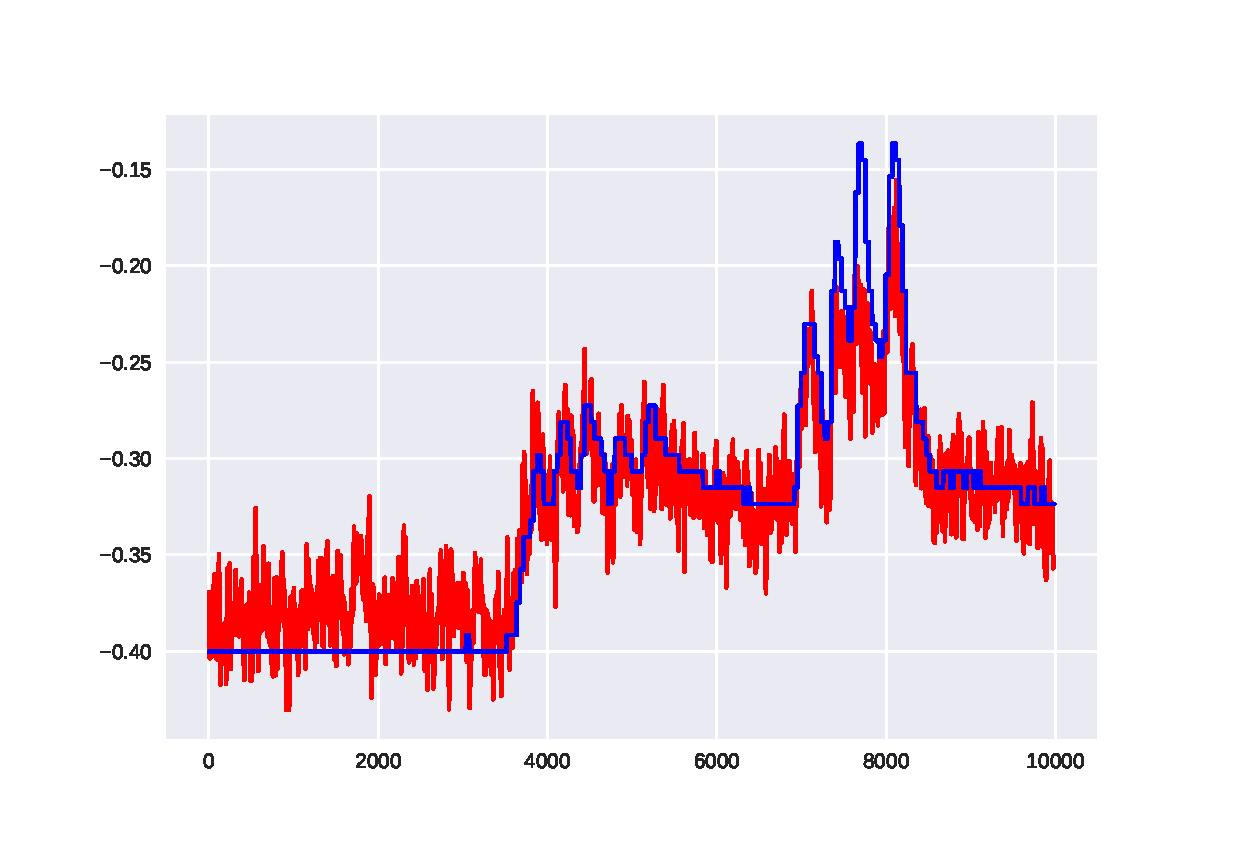
\includegraphics[width=\linewidth]{1.eps}
  \caption{Красный - фактический, синий - предсказанный}
  \label{fig:results}
\end{figure}
    
\section{Вывод}

\bibliographystyle{plain}
\bibliography{biblio}

\end{document}
